\monster{Muro Demoníaco}{8}{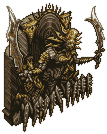
\includegraphics[width=0.17\textwidth]{./art/monsters/demonwall.png}}
{
 PV: & \hfill 250 & PM: & \hfill 200 \\
 FUE: & \hfill 9 & DEF: & \hfill 6 \\
 MAG: & \hfill 5 & RES: & \hfill 6 \\
 AGI: & \hfill 2 & Tamaño: & \hfill G\\
}
{
 \textbf{Espadas}: 3d de daño, 2u Alcance \hfill \textbf{Botín:} 2000 Gil \\
 \textbf{Inmune}: \hyperlink{status}{Todos los estados alterados} 
 
 \mtech{Morfeo++}{24}{2t}{2u}{5u}{
 Todos los enemigos que se encuentren en el área de efecto hacen una tirada con DC 8. Si fallan, \linebreak quedan \hyperlink{status}{Dormidos}. 
	}{\sleep} \mtech{Arremetida de Muro}{20}{1t}{10u (línea)}{Tú}{
 Arremetes hasta 10u hacia adelante en línea recta, infligiendo 8d de daño a todos los que estén en tu camino y los haces retroceder 3u. Si un enemigo queda aplastado entre ti y un muro, instantáneamente \linebreak pasan a estar \hyperlink{status}{KO}. 
}{\ko} 
\mpassive{Giro Brusco}{
 Cada vez que cambias de dirección, todos los que se encuentren a 2u reciben 6d de daño, pero no puedes realizar una acción en el mismo turno.
	}
	\vspace{0.1cm} \hrule \vspace{0.1cm} 
 "Como si las puertas asesinas no fueran suficientes..." -- Rydia
}

